\documentclass[12pt,a4paper]{article}
\usepackage[utf8]{inputenc}
\usepackage[english,italian]{babel}
\usepackage{amsmath}
\usepackage{amsfonts}
\usepackage{amssymb}
\usepackage{graphicx}
\usepackage[left=2cm,right=2cm,top=2cm,bottom=2cm]{geometry}
\title{FantaUnipa}
\author{Salvatore Calderaro \and Gaspare Casano}
\usepackage{hyperref}
\begin{document}
\date  {}
\maketitle
\thispagestyle{empty}
\newpage
\tableofcontents
\newpage
\selectlanguage{english}
\begin{abstract} 
FantaUnipa è un software che è stato creato per simulare il gioco del fantacalcio, scritto in linguaggio Java attraverso l'uso dell'IDE Eclipse e l'ausilio delle librerie Swing per l'implementazione delle interfacce grafiche. Per lo sviluppo sono stati utilizzati diversi Design Pattern e tramite l'utilizzo di essi è stato possibile creare un software funzionale e facilmente utilizzabile. 
\end{abstract}
\newpage
\selectlanguage{italian}
\section{Introduzione}
FantaUnipa è un software che permette la simulazione di un torneo del famoso gioco del fantacalcio. Il fantacalcio è un gioco che consiste nel creare e gestire squadre virtuali formate da calciatori reali, scelti fra quelli che giocano il campionato a cui il gioco si riferisce (ad esempio Serie A, Premier League, etc). Il software, dopo che l'utente ha effettuato la registrazione al sistema, crea gli altri cinque utenti virtuali che parteciperanno al torneo. La creazione degli utenti (virtuali e non) è stata implementata mediante l'utilizzo del design pattern strutturale \textit{Builder}. Questa scelta è giustificata dal fatto che,essendo la classe Fantallenatore formata da diversi attributi, il suo metodo costruttore avrebbe avuto troppi  passati a parametro; l'utilizzo del Builder ci ha permesso di costruire l'oggetto tramite l'utilizzo di appositi metodi per ogni singolo attributo.\\
Dopo avere effettuato la registrazione, l'utente dovrà inserire il nome e il logo della sua fantasquadra e parallelamente viene effettuata la stessa operazione per gli utenti virtuali. Una volta che tutti gli utenti hanno scelto il nome e il logo della loro fantasquadra inizia l'asta per l'acquisto dei giocatori. Ogni fantallenatore deve acquistare:
\begin{itemize}
\item 3 portieri;
\item 8 difensori;
\item 8 centrocampisti;
\item 6 attaccanti.
\end{itemize}
Durante le diverse sessioni dell'asta ogni partecipante può puntare, rilanciare o rinuciare a quel determinato giocatore.\\
L'asta è stata implementata mediante l'utilizzo dei design pattern comportamentali \textit{Observer} e \textit{Strategy}. In particolare Observer è stato utilizzato per notificare a tutti i fantallenatori (gli observer) il cambiamento di stato (valore della puntata, o un'eventuale rinuncia) dell'oggetto osservabile (sessione di asta per un determinato calciatore). In questo modo, in ogni momento, ogni fantallenatore è a conoscenza dello stato dell'asta e può decidere se rilanciare o abbandonare l'asta; strategy è stato utilizzato per implementare diverse strategie di rilancio utilizzate dagli utenti virtuali. In particolare è stato possibile cambiare a runtime il tipo di algoritmo da utilizzare in base alla strategia che ha deciso di adottare l'utente virtuale.\\
Dopo che tutti gli utenti hanno completato la creazione della propria rosa, il software genera il torneo composto da sei squadre che si sfideranno secondo la modalità del girone all'italiana. Per la creazione del torneo è stato utilizzato il pattern  Singleton ed il pattern strutturale Facade. Il pattern \textit{Singleton} è stato utilizzato per rendere l'entità torneo istanziabile una e una sola volta; \textit{Facade} è stato utilizzato per nascondere ai fantallenatori la   dell'entità torneo e per rendere più facile l'utilizzo dei sottosistemi da cui esso è composto.\\
Una volta creato il torneo, per ogni giornata, l'utente dovrà inserire la propria formazione scegliendo fra quattro diversi moduli disponibili (4-4-2, 4-3-3, 3-4-4, 3-5-2); la creazione della formazione per tutti gli utenti è stato implementato utilizzando il design pattern creazionale \textit{Factory method} il quale ci ha permesso di creare una classe (FormazioneFactory) che in base al tipo di modulo scelto dall'utente delega la creazione dell'oggetto alla sottoclasse corrispondente al modulo scelto.\\
Alla fine di ogni giornata l'utente avrà accesso ad una serie di informazioni inerenti il torneo (ad esempio classifica, risultati delle partite giocate etc).\\ Quando si conclude il torneo verranno visualizzate le squadre che si sono classificate nelle prime tre posizioni.
\section{Analisi e specifica dei requisiti}
\subsection{Stakeholder principali}
L'unico stakeholder del software FantaUnipa è il fantallenatore, che è colui che utilizza il software per simulare un torneo di fantacalcio. 
\subsection{Specifica dei requisiti funzionali}
Di seguito viene riportato l'elenco dei requisiti funzionali del fantallenatore:
\begin{itemize}
\item registrarsi al sistema;
\item effettuare il login;
\item creare la propria fantasquadra;
\item partecipare all'asta per l'acquisto dei giocatori;
\item gioca partita;
\item visualizzare il calendario del torneo;
\item visualizzare la propria rosa;
\item visualizzare la rosa degli altri fantallenatori;
\item visualizzare i voti e risultati delle partite precedenti;
\item visualizzare la classifica del torneo.
\end{itemize}
\subsection{Specifica dei requisiti NON funzionali}
Di seguito è riportata l'elenco dei requisiti non funzionali del sistema:
\begin{itemize}
\item usabilità: l'interfaccia utente è stata implementata cercando di garantire la massima usabilità ed una facile localizzazione dei comandi da utilizzare;
\item velocità: il software è stato progettato in modo tale da avere tempi di risposta brevi fra un'operazione ed un'altra;
\item portabilità: il software può essere eseguito su diversi sistemi;
\end{itemize}
\subsection{Casi d'uso}
\subsubsection{Registrazione al sistema}
Attore principale: \textbf{Fantallenatore}\\
\newline
\textbf{PASSI}
\begin{enumerate}
\item clicca sul bottone registrati;
\item il sistema visualizza il modulo per la registrazione;
\item l'utente compila tutti campi e preme il tasto registrati;
\item il sistema acquisisce e controlla i dati;
\item il sistema mostra un messaggio di conferma e visualizza il modulo di login.
\end{enumerate}
\textbf{ESTENSIONI}
\begin{enumerate}
\item uno o più campi vuoti: in questo caso viene mostrato all'utente un messaggio di errore e il sistema ritorna al passo 2;
\item la password non rispetta gli standard definiti dal sistema: in questo verrà mostrato all'utente un messaggio di errore e il sistema ritorna al passo 2;
\item l'username è stato già utilizzato: in questo caso verrà mostrato all'utente un messaggio di errore e il sistema ritorna al passo 2;
\end{enumerate}
\subsubsection{Effettuare il login}
Attore principale: \textbf{Fantallenatore}\\
\newline
\textbf{PASSI}
\begin{enumerate}
\item il sistema mostra all'utente il modulo per effettuare il login;
\item l'utente compila il modulo e clicca sul bottone login;
\item il sistema acquisisce e controlla i dati;
\item il sistema visualizza la schermata home del software nel caso in cui il fantallenatore avesse già creato la sua squadra, altrimenti viene visualizzata la schermata per la creazione della squadra.
\end{enumerate}
\textbf{ESTENSIONI}
\begin{itemize}
\item campi non validi: in questo caso il sistema visualizza un messaggio d'errore e torna al punto 1.
\end{itemize}
\subsubsection{Creazione squadra}
Attore principale: \textbf{Fantallenatore}\\
\newline
\textbf{PASSI}
\begin{enumerate}
\item il sistema visualizza il modulo per la creazione della squadra;
\item l'utente compila il modulo inserendo il nome della squadra ed il logo;
\item il sistema acquisisce i dati;
\item il sistema visualizza la finestra che permetterà all'utente di iniziare l'asta per la creazione della rosa.
\end{enumerate}
\textbf{ESTENSIONI}
\begin{itemize}
\item campi vuoti: il sistema visualizza un messaggio di errore e torna al punto 1.
\end{itemize}
\subsubsection{Partecipazione all'asta}
Attore principale: \textbf{Fantallenatore}\\
\newline
\textbf{PASSI}
\begin{enumerate}
\item il sistema visualizza una finestra che consente all'utente di ricercare i giocatori che intende acquistare
\item l'utente  a questo punto può:
\begin{itemize}
\item inserire il nome del giocatore nell'apposito campo e premere il bottone cerca: in questo caso gli verrà mostrato il nome del giocatore e il bottone scegli
\item premere il bottone Mostra Tutti e cliccare su uno dei giocatori della lista.
\end{itemize}
\item in entrambi i casi precedenti dopo il click il sistema visualizzerà una finestra in cui si svolgeranno le operazioni per l'asta;
\item l'utente inserisce la puntata e clicca su punta;
\item il sistema visualizza le puntate degli altri giocatori;
\item l'utente può decidere se rinunciare cliccando sul bottone rinuncia o se effettuare una nuova puntata.
\end{enumerate}
\textbf{ESTENSIONI}
\begin{itemize}
\item il giocatore scelto è stato già acquistato oppure l'utente non ha inserito il nome di alcun giocatore: in questo caso viene mostrata una finestra di notifica e il sistema ritorna la punto 1;
\item puntata non consentita: il sistema mostra una finestra di errore e ritorna al punto 3;
\item l'utente si aggiudica il giocatore: il sistema visualizza un messaggio di conferma e torna al punto 1.
\end{itemize}
\subsubsection{Gioca partita}
Attore principale: \textbf{Fantallenatore}\\
\newline
\textbf{PASSI}
\begin{enumerate}
\item nella schermata Home l'utente clicca sul bottone schiera formazione;
\item il sistema visualizza una finestra per la scelta del modulo;
\item l'utente clicca su una delle voci del menù a tendina;
\item il sistema visualizza una finestra dove l'utente potrà scegliere i singoli giocatori da schierare;
\item l'utente dopo aver scelto sia i titolari che le riserve clicca su conferma;
\item il sistema  una finestra contenente i risultati della giornata e dei bottoni (visualizza voti) che permettono all'utente di visualizzare i voti ottenuti dai giocatori in una determinata partita;
\item se l'utente clicca su visualizza voti il sistema mostra una finestra con i voti dei giocatori per quella determinata partita;
\item l'utente dopo aver chiuso la finestra ritorna al punto 1.
\end{enumerate}
\textbf{ESTENSIONI}
\begin{itemize}
\item se l'utente inserisce un giocatore più di una volta oppure lascia uno o più campo vuoti, il sistema visualizza un messaggio di errore e ritorna al punto 4;
\end{itemize}
\subsubsection{Visualizzare il calendario del torneo}
Attore principale: \textbf{Fantallenatore}\\
\newline
\textbf{PASSI}
\begin{enumerate}
\item l'utente nella schermata home clicca sul bottone calendario;
\item il sistema mostra una finestra contenente dei bottoni inerenti le cinque giornate;
\item l'utente clicca su uno dei cinque bottoni;
\item il sistema mostra una finestra in cui sono contenute le partite della giornata con il risultato e un tasto che permette di visualizzare le informazioni, qualora la giornata si fosse già giocata;
\item quando l'utente chiude la finestra il sistema ritorna al punto 1;
\end{enumerate}
\subsubsection{Visualizzare la propria rosa}
Attore principale: \textbf{Fantallenatore}\\
\newline
\textbf{PASSI}
\begin{enumerate}
\item l'utente dalla schermata home clicca sul bottone visualizza la mia rosa;
\item il sistema visualizza una finestra contenente la lista di tutti i giocatori che compongono la rosa dell'utente;
\end{enumerate}
\subsubsection{Visualizzare la rosa delle altre squadre}
Attore principale: \textbf{Fantallenatore}\\
\newline
\textbf{PASSI}
\begin{enumerate}
\item l'utente dalla schermata home clicca sul bottone visualizza la mia rosa;
\item il sistema visualizza una finestra contenente i loghi di tutte le altre squadre che partecipano al torneo;
\item l'utente clicca su uno dei loghi;
\item il sistema visualizza una finestra che mostra la rosa della squadra corrispondente al logo su cui ha cliccato l'utente.
\end{enumerate}
\subsubsection{Visualizzare i voti e i risultati delle partite precedenti}
Attore principale: \textbf{Fantallenatore}\\
\newline
\textbf{PASSI}
\begin{enumerate}
\item l'utente dalla schermata home clicca sul bottone calendario;
\item il sistema mostra una finestra contenente dei bottoni inerenti le cinque giornate;
\item l'utente clicca sul bottone corrispondente alla giornata di cui intende visualizzare le informazioni;
\item il sistema mostra una finestra contenente i risultati delle partite e qualora le partite fossero state già giocate un tasto info;
\item l'utente clicca sul tasto info;
\item il sistema mostra una finestra contenente i voti ottenuti dai giocatori in quella determinata partita; 
\end{enumerate}
\subsubsection{Visualizza classifica}
Attore principale: \textbf{Fantallenatore}\\
\newline
\textbf{PASSI}
\begin{enumerate}
\item l'utente dalla schermata home clicca sul bottone classifica;
\item il sistema mostra una finestra contenente la classifica corrente del torneo.
\end{enumerate}
\newpage
\section{Diagrammi UML dell'architettura software}
\subsection{Diagrammi dei casi d'uso}
Il diagramma dei casi d'uso di seguito riportato rappresenta la mappa riassuntiva dei casi d'uso  e riporta per l'unico l'attore (il fantallenatore) tutte le azioni che esso può compiere.
\begin{figure}[h]
\centering
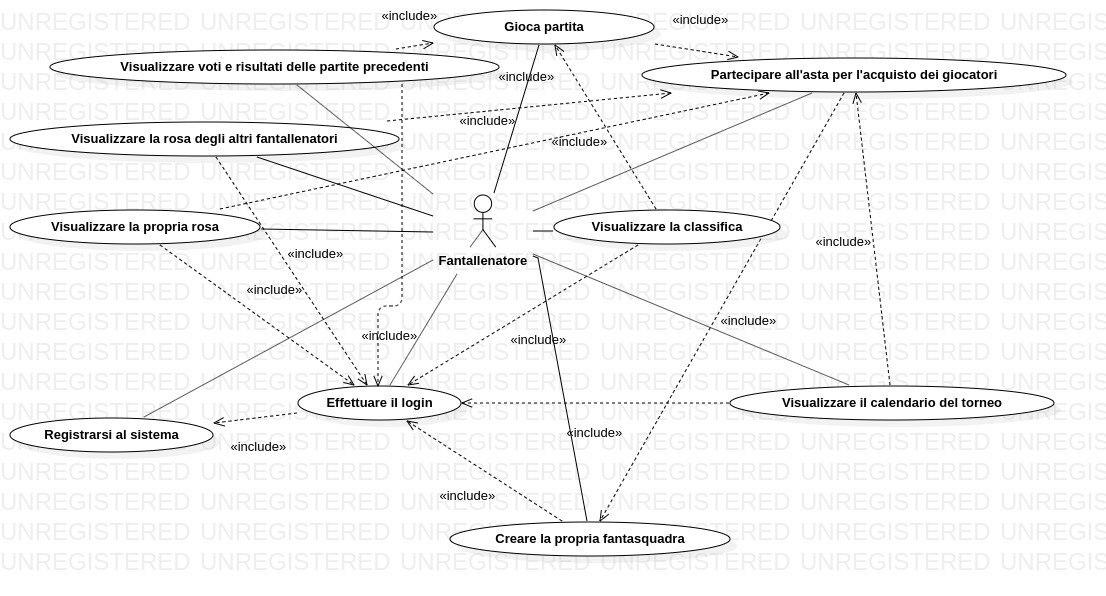
\includegraphics[width=15 cm,keepaspectratio]{diagrammaCasiUso.jpg}
\caption{Diagramma dei casi d'uso}
\end{figure}
\subsection{Diagramma UML delle classi}
Di seguito è riportato il diagramma UML delle classi completo.
\begin{figure}[h]
\centering
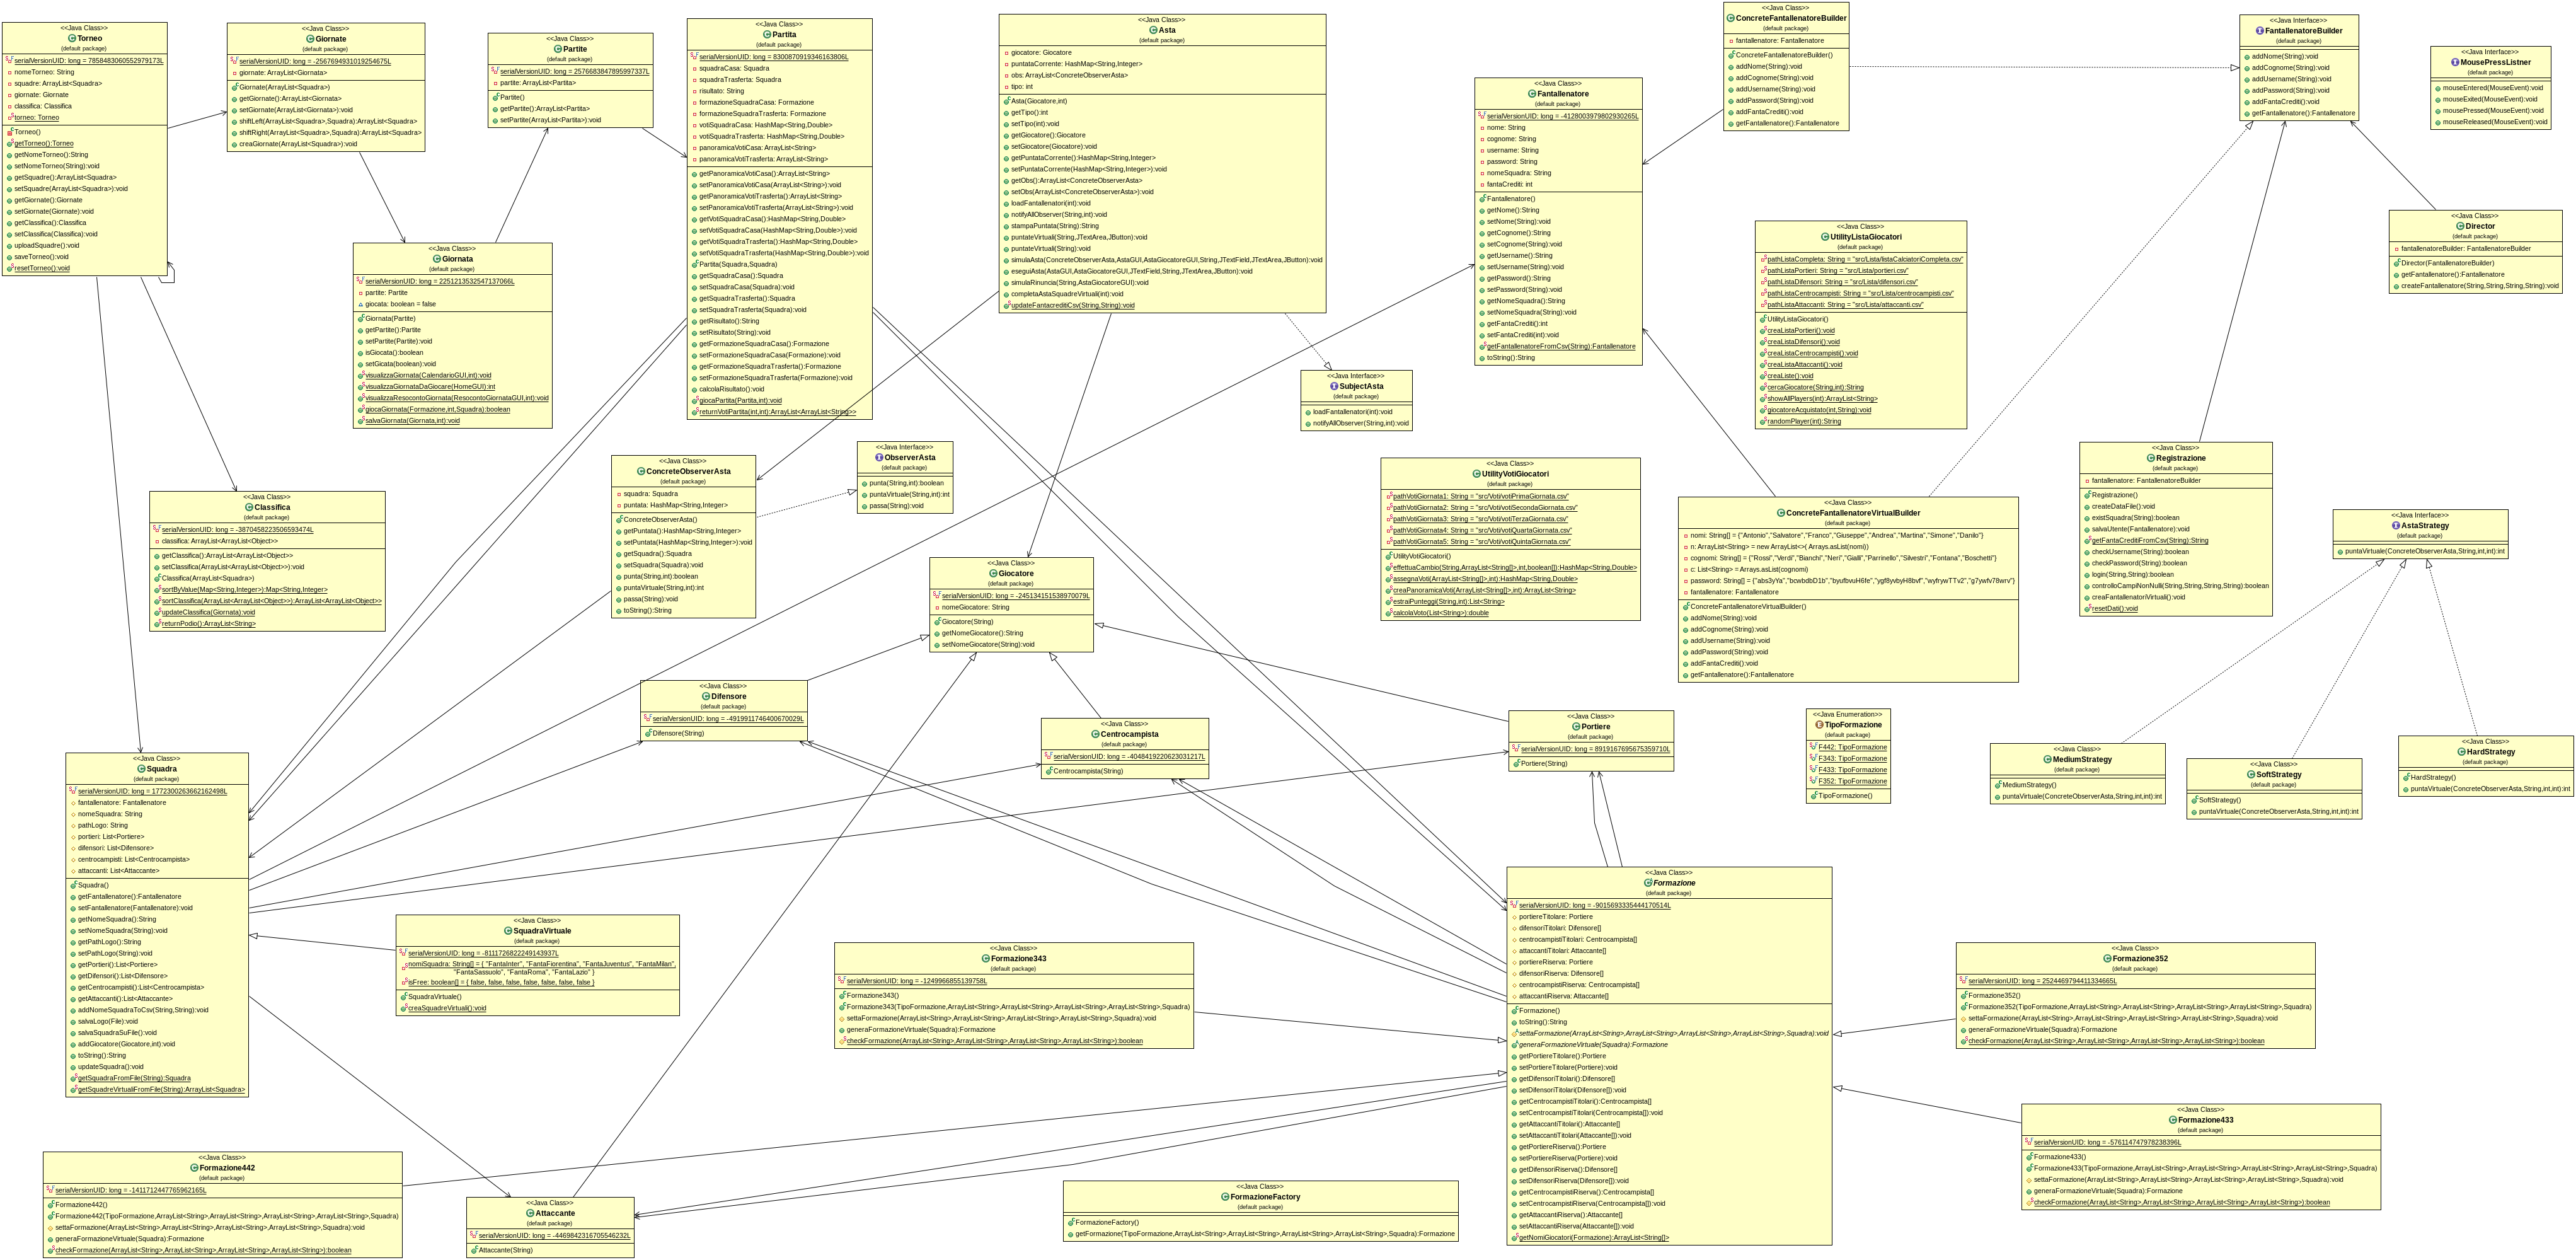
\includegraphics[width=15 cm,keepaspectratio]{FANTAUNIPA.png}
\caption{Diagramma UML}
\end{figure}
\section{Design pattern utilizzati}
 In questa sezione vengono mostrati i design pattern utilizzati per lo sviluppo del software.
 \subsection{Pattern creazionali}
 \subsubsection{Singleton}
 Il design pattern Singleton crea e gestisce un'istanza di una classe che si vuole rendere istanziabile una sola volta. Ciò si ottiene marcando il costruttore come private in modo tale che non possano essere creati oggetti da classi esterne  e poiché l'oggetto è statico per quella classe, l'unico modo per ottenere l'accesso ad esso è  mediante  un metodo static \textit{getIstance()}.
 \begin{figure}[h]
\centering
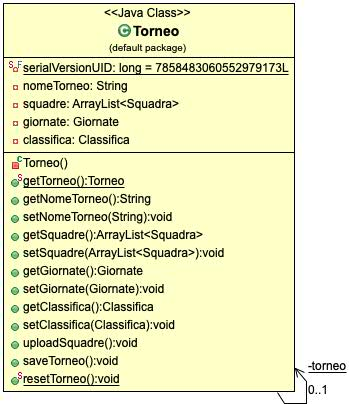
\includegraphics[width=11 cm,keepaspectratio]{Singleton.jpg}
\caption{Classe Singleton Torneo}
\end{figure}
Nello sviluppo di  questo software è stato utilizzato tale pattern per la creazione della classe \textbf{Torneo}, la quale deve essere istanziata una sola volta e  deve poter essere non istanziabile da classi esterne ad essa, in quanto nel gioco del fantacalcio non possono coesistere due o più tornei per volta.
\newpage
\subsubsection{Builder}
Il design pattern Builder viene utilizzato  per la costruzione di un oggetto complesso,  in particolar separa quest'ultimo dalla sua rappresentazione in modo tale che il processo costruzione stesso possa creare diverse rappresentazioni. Esso rappresenta una valida alternativa ai costruttori. Esso si realizza creando un oggetto \textbf{Director}  che viene configurato con gli oggetti 	\textbf{Builder} che si intendono costruire. Il Director notifica al Builder se una parte del prodotto deve essere costruita, e il Builder ricevuta la richiesta aggiunge la parte al prodotto. \\
 \begin{figure}[h]
\centering
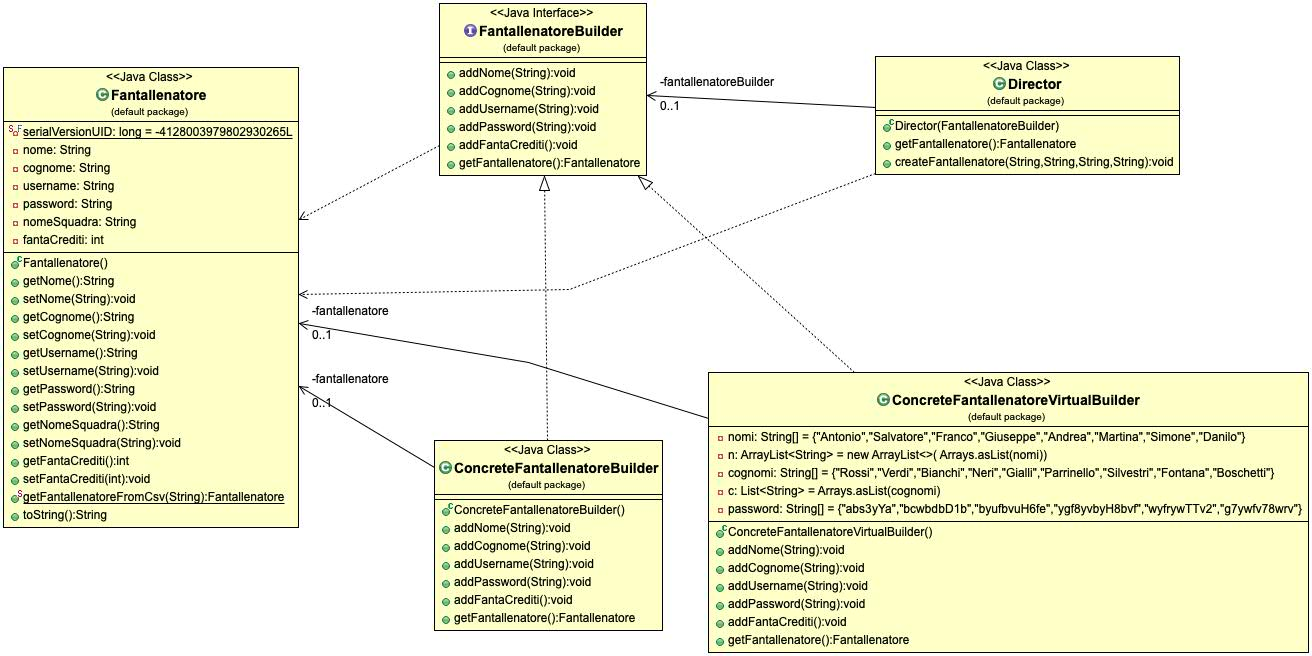
\includegraphics[width=15 cm,keepaspectratio]{Builder.jpg}
\caption{Classi coinvolte nell'implementazione del Builder}
\end{figure}
\newline
Nello sviluppo di questo software tale pattern è stato utilizzato per la costruzione dell'oggetto \textbf{Fantallenatore}, il quale è formato da tanti attributi e necessita di vari step per la sua costruzione; inoltre è stato utilizzato per differenziare la creazione del fantallenatore (l'utente reale) e il fantallenatore virtuale il quale viene costruito in maniera differente rispetto al primo. Le classi coinvolte nell'implementazione di tale pattern sono:
\begin{itemize}
\item \textbf{Fantallenatore}: è l'oggetto che deve essere costruito (Product) ;
\item \textbf{FantallenatoreBuilder}: interfaccia in cui vengono dichiarati  i metodi che serviranno per la costruzione dell'oggetto (Builder);
\item \textbf{ConcreteFantallenatoreBuilder}: concretizzazione del FantallenatoreBuilder che implementa i metodi per la costruzione del fantallenatore reale (ConcreteBuilder);
\item \textbf{ConcreteFantallenatoreVirtuale}: concretizzazione del FantallenatoreBuilder che implementa i metodi per la costruzione del fantallenatore virtuale (ConcreteBuilder);
\item \textbf{Director}: classe che dirige la costruzione degli oggetti.
\end{itemize}
\newpage
\subsubsection{Factory method}
Il pattern FactoryMethod consiste nel delegare la costruzione di un oggetto ad una factory; viene definita una classe astratta o interfaccia per la creazione dell'oggetto e di conseguenza le sue concretizzazioni possono decidere quale classe istanziare.
\begin{figure}[h]
\centering
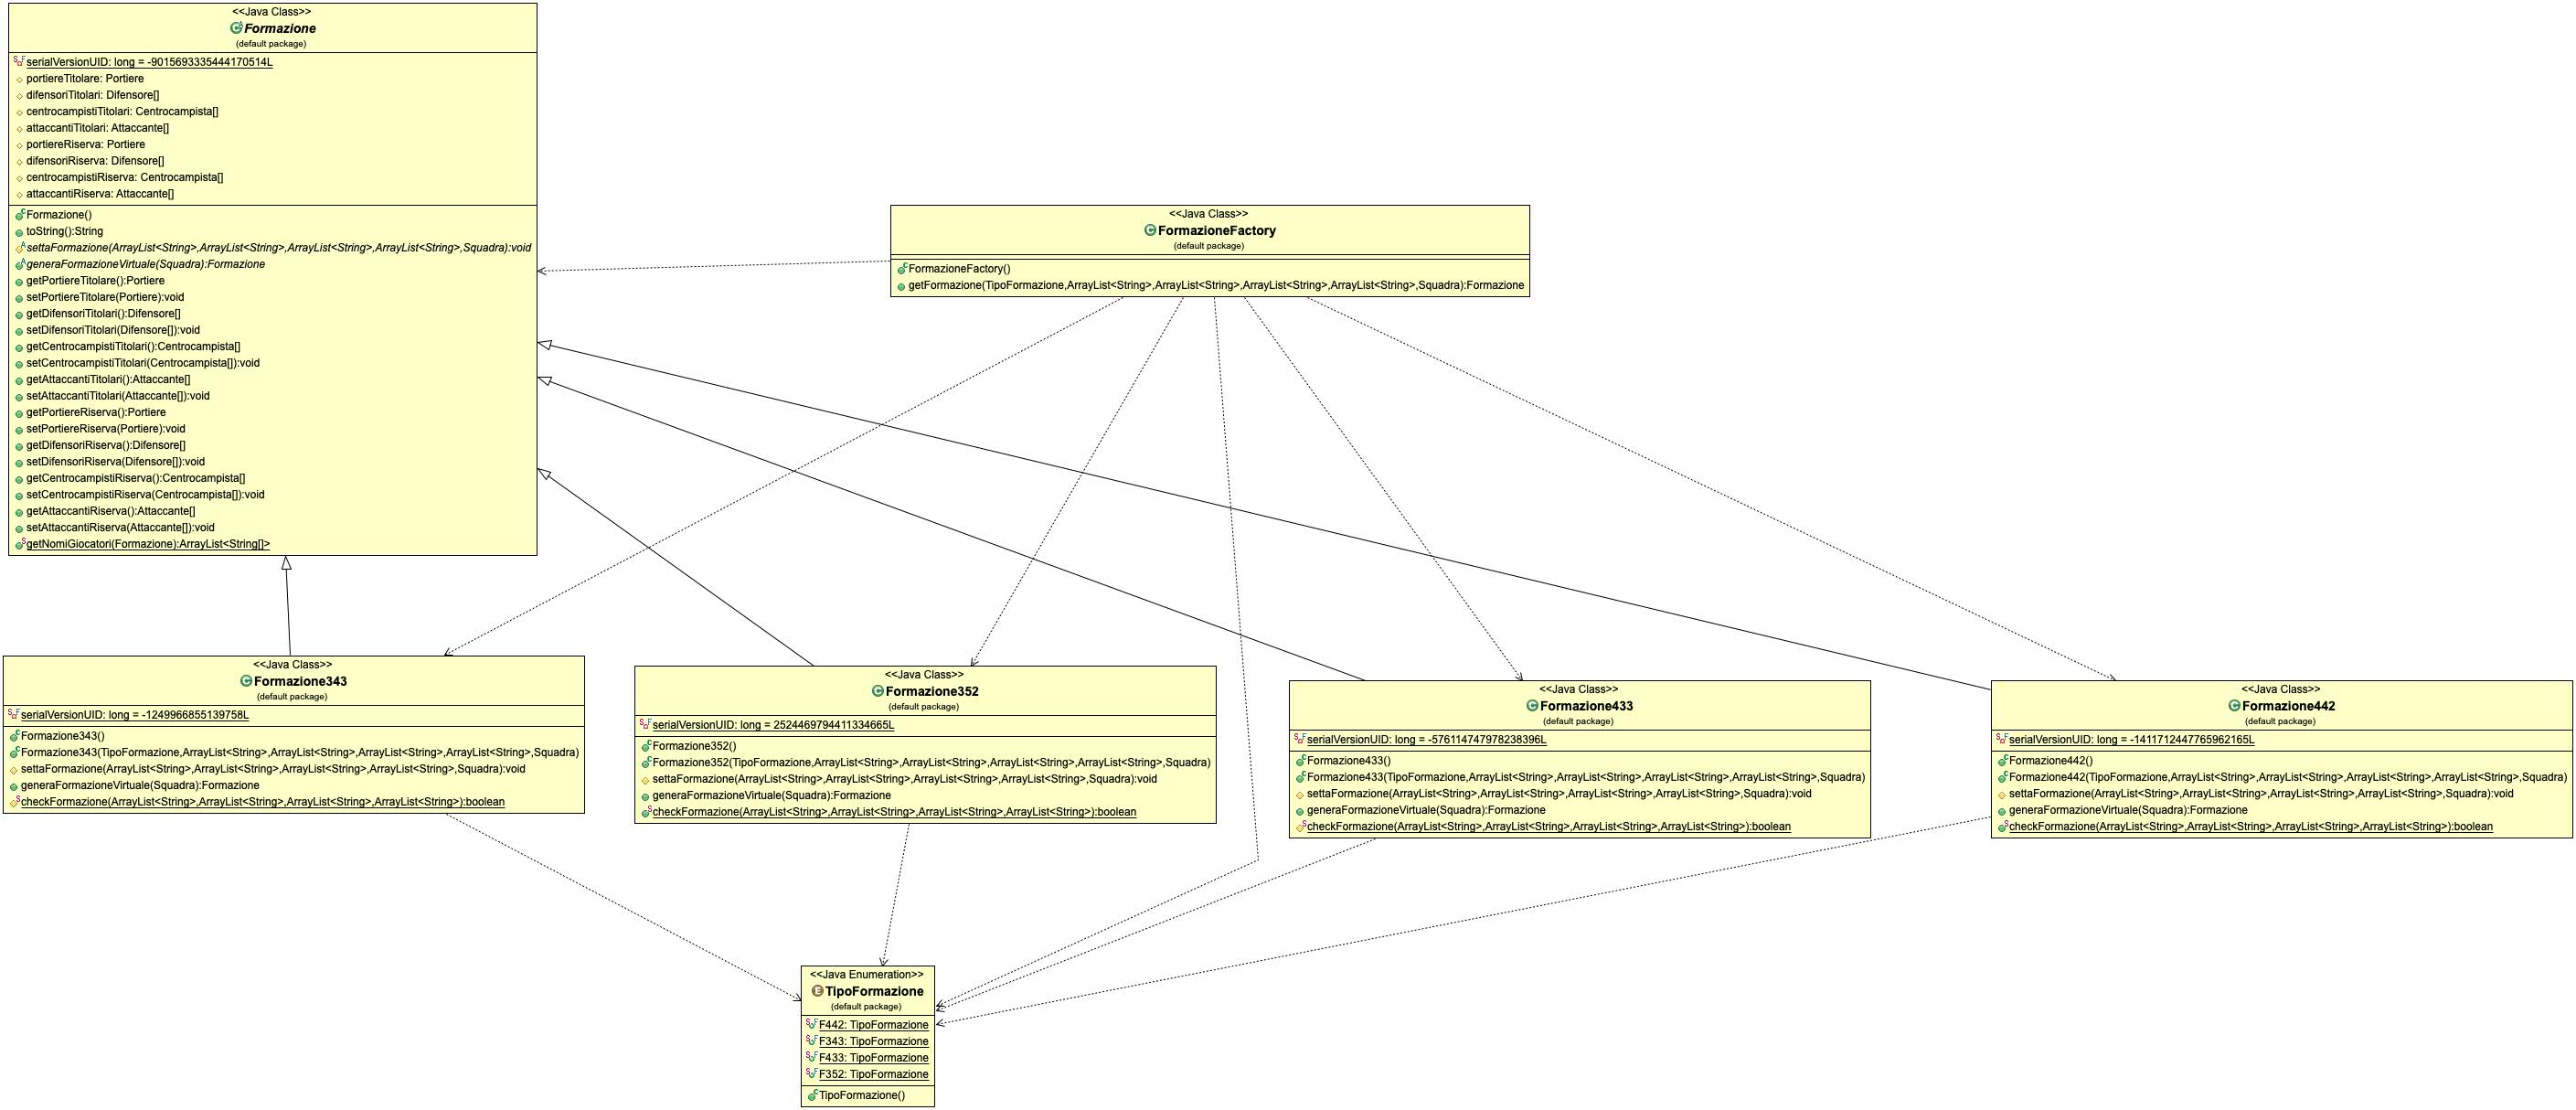
\includegraphics[width=18 cm ,keepaspectratio]{Factory.jpg}
\caption{Classi coinvolte nell'implementazione del Factory method}
\end{figure}
\newline
Nello sviluppo di questo software tale pattern è stato utilizzato per la costruzione dell'oggetto \textbf{Formazione}; data la necessità di avere diversi moduli per la formazione tramite la factory è stato possibile creare l'oggetto formazione delegandone la costruzione alle sue sottoclassi. Le classi coinvolte sono:  
\begin{itemize}
\item \textbf{FormazioneFactory}: classe che contiene il factory method per la costruzione dell'oggetto formazione (Creator);
\item \textbf{Formazione}: classe astratta dell'oggetto concreto che il factory method genera, che dichiara il metodo per il settaggio della formazione (Product);
\item \textbf{Formazione442}: concretizzazione della classe Formazione  (ConcreteProduct);
\item \textbf{Formazione433}: concretizzazione della classe Formazione  (ConcreteProduct);
\item \textbf{Formazione343}: concretizzazione della classe Formazione  (ConcreteProduct);
\item \textbf{Formazione352}: concretizzazione della classe Formazione  (ConcreteProduct);
\item \textbf{TipoFormazione}: enum usata per definire il tipo di formazione.
\end{itemize}
\newpage
\subsection{Pattern comportamentali}
\subsubsection{Observer}
Il pattern comportamentale Observer definisce una dipendenza uno a molti tra gli oggetti in modo che quando un oggetto cambia stato, tutti i suoi osservatori vengono avvisati e aggiornati automaticamente. Il cambiamento di stato di un oggetto osservabile viene notificato agli oggetti che sono registrati dall'osservatore. Esso si realizza   mediante un'interfaccia Subject che dichiara i metodi dell'oggetto osservabile e un'interfaccia Observer che dichiara i metodi degli osservatori. Quest'ultime vengono concretizzate in due rispettive classi ConcreteSubject e ConcreteObserver; sarà compito della classe  ConcreteSubject notificare il cambio di stato dell'oggetto a tutti gli osservatori ad essa registrati, mentre sarà compito della classe ConcreteObserver definire il comportamento in caso di cambio di stato dell'oggetto osservato.
\begin{figure}[h]
\centering
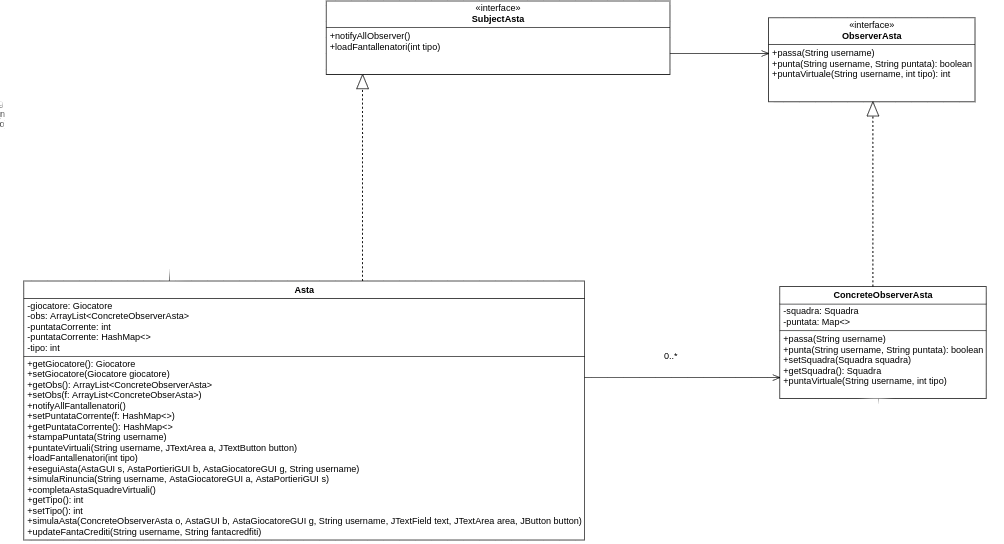
\includegraphics[width=18 cm ,keepaspectratio]{Observer}
\caption{Classi coinvolte nell'implementazione dell'Observer}
\end{figure}
\newline
Nello sviluppo di questo software tale pattern è stato utilizzato per implementare l'asta tra i fantallenatori  per la composizione della rosa. Grazie a tale pattern ogni fantallenatore, durante l'asta, è a conoscenza dei fantallenatori  che stanno partecipando  e delle loro rispettive puntate. Ogni volta che un fantallenatore effettua una nuova puntata, rinuncia all'asta o si aggiudica un giocatore queste informazioni vengono notificate a tutti gli osservatori.  Le classi coinvolte sono:
\begin{itemize}
\item \textbf{SubjectAsta}: interfaccia che dichiara i metodi per caricare i fantallentori che parteciperanno all'asta e un metodo che notifica le informazioni inerenti l'asta a tutti gli osservatori registrati;
\item \textbf{Asta}: concretizzazione di SubjectAsta, usata per la gestione delle operazioni inerenti l'asta;
\item \textbf{ObserverAsta}: interfaccia che dichiara i metodi che permettono al fantallenatore (Observer) di effettuare la puntata o rinunciare;
\item \textbf{ConcreteObserverAsta}: concretizzazione di ObserverAsta contenente le principali operazioni svolte dal Fantallenatore durante l'asta.
\end{itemize}
\subsubsection{Strategy}
Il pattern comportamentale Strategy serve a definire una famiglia di algoritmi da utilizzare per una stessa famiglia di oggetti rendendoli intercambiabili fra di loro. Strategy consente all'algoritmo di variare indipendentemente dai client che lo utilizzano. Tale pattern viene utilizzato quando è utile cambiare a dinamicamente  gli algoritmi utilizzati da un'applicazione. 
\begin{figure}[h]
\centering
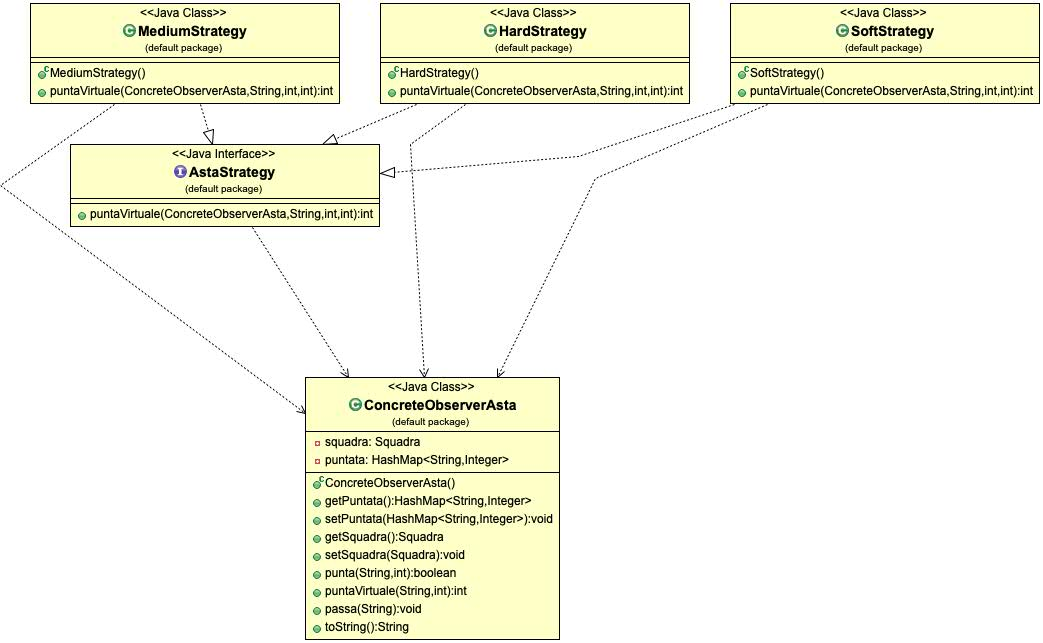
\includegraphics[width=18 cm ,keepaspectratio]{Strategy}
\caption{Classi coinvolte nell'implementazione di Strategy}
\end{figure}
\newline
Nello sviluppo di questo software tale pattern è stato utilizzato per implementare diverse strategie che un fantallenatore virtuale può adottare durante una sessione d'asta. Le classi coinvolte sono:
\begin{itemize}
\item \textbf{AstaStrategy}: interfaccia che dichiara il metodo \textit{puntaVirtuale} che consente ai fantallenatori virtuali di effettuare la puntata;
\item \textbf{SoftStrategy}: concretizzazione di AstaStrategy in cui il metodo \textit{puntaVirtuale} viene implementato in modo tale che il fantallenatore rilanci di uno rispetto all'offerta massima;
\item \textbf{MediumStrategy}: concretizzazione di AstaStrategy in cui il metodo \textit{puntaVirtuale} viene implementato in modo tale che il fantallenatore rilanci di cinque rispetto all'offerta massima;
\item \textbf{HardStrategy}: concretizzazione di AstaStrategy in cui il metodo \textit{puntaVirtuale} viene implementato in modo tale che il fantallenatore rilanci di dieci rispetto all'offerta massima;
\item \textbf{ConcreteObserverAsta}: osservatore che partecipa all'asta che a runtime utilizza una di queste strategie.

\end{itemize}
\subsection{Pattern strutturali}
\subsubsection{Facade}
Il pattern strutturale Facade si utilizza per nascondere la complessità di un sottosistema complesso al client. Esso fornisce un'interfaccia unificata a un set di interfacce in un sottosistema. Facade definisce un'interfaccia di alto livello che semplifica l'utilizzo del sottosistema.
\begin{figure}[h]
\centering
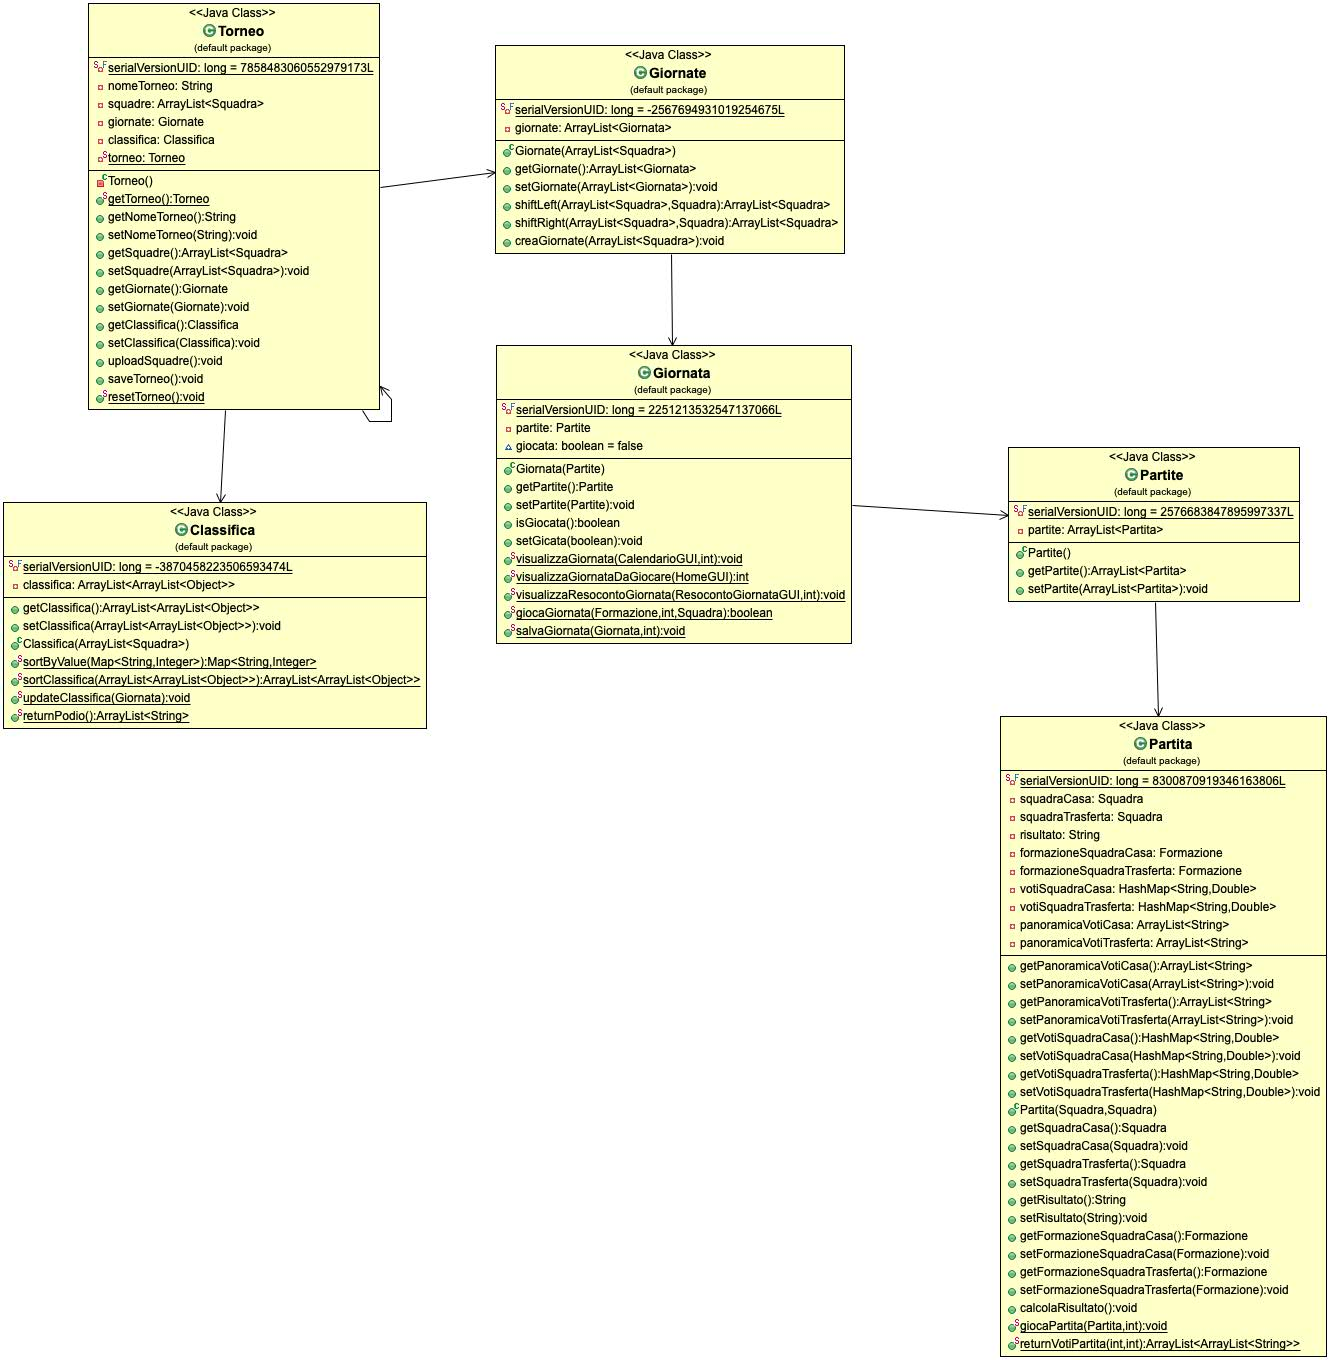
\includegraphics[width=16 cm ,keepaspectratio]{Facade.jpg}
\caption{Classi coinvolte nell'implementazione di Facade}
\end{figure}
\newline
Nello sviluppo di questo software tale pattern è stato utilizzato per l'implementazione del sistema Torneo , il quale rappresenta un'entità complessa. In particolar modo è stato usato per la nascondere la complessità dei sottosistemi al client. Le classi coinvolte sono:
\begin{itemize}
\item \textbf{Torneo}: classe Facade che contiene i vari metodi per la gestione del torneo;
\item \textbf{Classifica}: classe per la gestione della Classifica del torneo;
\item \textbf{Giornate}: classe per al gestione di tutte le giornate che compongono il torneo;
\item \textbf{Giornata}: classe per la gestione di una singola giornata del torneo;
\item \textbf{Partite}: classe per la gestione di tutte le partite di una giornata;
\item \textbf{Partita}: classe per la gestione di una singola partita.
\end{itemize}
\section{Conclusioni}
FantaUnipa è un software che può definirsi una simulazione del gioco del FantaCalcio, in quanto chi utilizza il software può partecipare ad un torneo competendo soltanto con utenti virtuali. Tuttavia, grazia alle tecniche utilizzate durante l'implementazione, sarà possibile in futuro aggiunge diverse nuove funzionalità per ampliare le funzionalità come:
\begin{itemize}
\item creazione di una web API per far partecipare al gioco solamente utenti reali;
\item ampliazione del torneo con simulazione dell'intero campionato di riferimento scelto;
\item aggiunta di due aste di riparazione per il mercato estivo ed invernale;
\item aggiornamento live dei voti durante le partite reali.
\end{itemize}
\end{document}
